% Options for packages loaded elsewhere
\PassOptionsToPackage{unicode}{hyperref}
\PassOptionsToPackage{hyphens}{url}
%
\documentclass[
  12pt,
]{article}
\usepackage{lmodern}
\usepackage{amssymb,amsmath}
\usepackage{ifxetex,ifluatex}
\ifnum 0\ifxetex 1\fi\ifluatex 1\fi=0 % if pdftex
  \usepackage[T1]{fontenc}
  \usepackage[utf8]{inputenc}
  \usepackage{textcomp} % provide euro and other symbols
\else % if luatex or xetex
  \usepackage{unicode-math}
  \defaultfontfeatures{Scale=MatchLowercase}
  \defaultfontfeatures[\rmfamily]{Ligatures=TeX,Scale=1}
\fi
% Use upquote if available, for straight quotes in verbatim environments
\IfFileExists{upquote.sty}{\usepackage{upquote}}{}
\IfFileExists{microtype.sty}{% use microtype if available
  \usepackage[]{microtype}
  \UseMicrotypeSet[protrusion]{basicmath} % disable protrusion for tt fonts
}{}
\makeatletter
\@ifundefined{KOMAClassName}{% if non-KOMA class
  \IfFileExists{parskip.sty}{%
    \usepackage{parskip}
  }{% else
    \setlength{\parindent}{0pt}
    \setlength{\parskip}{6pt plus 2pt minus 1pt}}
}{% if KOMA class
  \KOMAoptions{parskip=half}}
\makeatother
\usepackage{xcolor}
\IfFileExists{xurl.sty}{\usepackage{xurl}}{} % add URL line breaks if available
\IfFileExists{bookmark.sty}{\usepackage{bookmark}}{\usepackage{hyperref}}
\hypersetup{
  pdftitle={Hurricane Michael and Floridian Turnout},
  pdfauthor={Kevin Morris; Peter Miller},
  hidelinks,
  pdfcreator={LaTeX via pandoc}}
\urlstyle{same} % disable monospaced font for URLs
\usepackage[margin=1in]{geometry}
\usepackage{longtable,booktabs}
% Correct order of tables after \paragraph or \subparagraph
\usepackage{etoolbox}
\makeatletter
\patchcmd\longtable{\par}{\if@noskipsec\mbox{}\fi\par}{}{}
\makeatother
% Allow footnotes in longtable head/foot
\IfFileExists{footnotehyper.sty}{\usepackage{footnotehyper}}{\usepackage{footnote}}
\makesavenoteenv{longtable}
\usepackage{graphicx}
\makeatletter
\def\maxwidth{\ifdim\Gin@nat@width>\linewidth\linewidth\else\Gin@nat@width\fi}
\def\maxheight{\ifdim\Gin@nat@height>\textheight\textheight\else\Gin@nat@height\fi}
\makeatother
% Scale images if necessary, so that they will not overflow the page
% margins by default, and it is still possible to overwrite the defaults
% using explicit options in \includegraphics[width, height, ...]{}
\setkeys{Gin}{width=\maxwidth,height=\maxheight,keepaspectratio}
% Set default figure placement to htbp
\makeatletter
\def\fps@figure{htbp}
\makeatother
\setlength{\emergencystretch}{3em} % prevent overfull lines
\providecommand{\tightlist}{%
  \setlength{\itemsep}{0pt}\setlength{\parskip}{0pt}}
\setcounter{secnumdepth}{5}
\usepackage{rotating}
\usepackage{setspace}
\newcommand{\beginsupplement}{\setcounter{table}{0}  \renewcommand{\thetable}{A\arabic{table}} \setcounter{figure}{0} \renewcommand{\thefigure}{A\arabic{figure}}}
\usepackage{booktabs}
\usepackage{longtable}
\usepackage{array}
\usepackage{multirow}
\usepackage{wrapfig}
\usepackage{float}
\usepackage{colortbl}
\usepackage{pdflscape}
\usepackage{tabu}
\usepackage{threeparttable}
\usepackage{threeparttablex}
\usepackage[normalem]{ulem}
\usepackage{makecell}
\usepackage{xcolor}
\newlength{\cslhangindent}
\setlength{\cslhangindent}{1.5em}
\newenvironment{cslreferences}%
  {\setlength{\parindent}{0pt}%
  \everypar{\setlength{\hangindent}{\cslhangindent}}\ignorespaces}%
  {\par}

\title{Hurricane Michael and Floridian Turnout\thanks{The authors thanks Many People for their comments on this project. All errors are our responsibility.}}
\author{Kevin Morris\footnote{Researcher, Brennan Center for Justice at NYU School of Law, 120 Broadway Ste 1750, New York, NY 10271 (\href{mailto:kevin.morris@nyu.edu}{\nolinkurl{kevin.morris@nyu.edu}})} \and Peter Miller\footnote{Researcher, Brennan Center for Justice at NYU School of Law, 120 Broadway Ste 1750, New York, NY 10271 (\href{mailto:peter.miller@nyu.edu}{\nolinkurl{peter.miller@nyu.edu}})}}
\date{April 24, 2020}

\begin{document}
\maketitle
\begin{abstract}
The United States is facing unprecedented challenges to election administration from the novel coronavirus. In response, many election administrators and advocates are calling for expanded vote-by-mail options to reduce in-person voting. To test the efficacy of loosened vote-by-mail rules we look to the experience of Florida in 2018, when Hurricane Michael devastated parts of the panhandle. By leveraging cross-jurisdiction variation in loosened restrictions in a double-matched triple-differences model, we show that loosened restrictions on vote-by-mail alone were not successful at eliminating administrative costs to voting. As administrators around the country loosen mail-voting restrictions in advance of this fall, they must couple these eased restrictions with strong public education campaigns about how voters can take advantange of them.
\end{abstract}

\pagenumbering{gobble}
\pagebreak

\pagenumbering{arabic}
\doublespacing

\hypertarget{research-design-and-expectations}{%
\section*{Research Design and Expectations}\label{research-design-and-expectations}}
\addcontentsline{toc}{section}{Research Design and Expectations}

Based on prior research, we expect that turnout was substantially depressed in the treated counties in 2018. This depressed turnout, however, was likely caused by both individual- and administrative-level mechanisms.

\hypertarget{individual-level-effects}{%
\subsection*{Individual-Level Effects}\label{individual-level-effects}}
\addcontentsline{toc}{subsection}{Individual-Level Effects}

We know that Hurricane Michael caused substantial destruction; as discussed in the introduction to this paper, residents lost their lives, flooding was widespread, and the hurricane caused billions of dollars of property damage. Would-be voters were now faced with myriad disruptions to their daily lives; it is likely that the direct effects of the weather, therefore, reduced turnout substantially. As professor emeritus Robert Montjoy told NPR in the aftermath of the storm, ``Whether casting a ballot becomes a higher priority than cleaning out the basement, visiting someone in the hospital, or all the other demands\ldots You certainly expect a lower turnout for those reasons'' (Parks \protect\hyperlink{ref-Parks2018}{2018}).

\hypertarget{administrative-effects}{%
\subsection*{Administrative Effects}\label{administrative-effects}}
\addcontentsline{toc}{subsection}{Administrative Effects}

The hurricane also caused problems for county election administrators, as the reporting around the Governor's executive order makes clear.\footnote{Executive Order 18-283 can be found here: \url{https://www.flgov.com/wp-content/uploads/2018/10/SLT-BIZHUB18101809500.pdf}. In the event that this link no longer works, it is on file with the authors.} Polling places were destroyed; some mail voters were residing in locations other than their registered addresses; would-be poll workers were unavailable. These factors could have increased the costs of voting even for residents who were not directly impacted by the hurricane, and increased the costs of voting even more for individuals who were directly impacted. Absent mitigation, the administrative effects of Hurricane Michael likely would have decreased turnout above-and-beyond the individual effects of the storm.

Executive Order 18-283 sought to offset the administrative barriers to voting by allowing county election administrators to flexibly respond to the damage wrought by the storm. Specifically, Executive Order 18-283 allowed administrators to add early voting locations; begin early voting 15 days before the general election, and continue until the day of the election; to accept vote-by-mail requests to addresses other than a voter's registered address; to send vote-by-mail ballots by forwardable mail; to deliver vote-by-mail ballots to electors or electors' immediate family members on election day without an affidavit; to relocate or consolidate polling places; and required poll watchers to be registered by the second Friday before the general election.

This paper sets out to answer two questions: what was the total depressive effect of the hurricane? And did Executive Order 18-283 effectively offset the depressive administrative effects?

\hypertarget{estimating-the-net-effects-of-the-hurricane}{%
\subsection*{Estimating the Net Effects of the Hurricane}\label{estimating-the-net-effects-of-the-hurricane}}
\addcontentsline{toc}{subsection}{Estimating the Net Effects of the Hurricane}

We begin by testing the net effect of each of these treatments on individual-level turnout. Our central identification strategy involves the use of difference-in-differences models. By comparing historical and 2018 turnout for voters in the counties hit by the storm to historical and 2018 turnout of voters elsewhere in the state, we can estimate the effect of the storm on turnout. To ensure a high-quality difference-in-differences specification, we do not include all untreated voters in our control group; rather, we match each treated voter with five untreated voters along a battery of individual- and neighborhood-level characteristics. Untreated voters who do not serve as matches are excluded from our models. Although it may seem counterintuitive to exclude data from our models, this matching procedure substantially improves the parallel trends assumptions necessary for a rigorous difference-in-differences analysis.

This design allows us to test our first hypothesis:

\textbf{Hypothesis 1:} Turnout in the eight treated counties was lower in 2018 due to the combined effects of the hurricane, county-level responses, and the executive order.

\hypertarget{testing-adminstrative-effects}{%
\subsection*{Testing Adminstrative Effects}\label{testing-adminstrative-effects}}
\addcontentsline{toc}{subsection}{Testing Adminstrative Effects}

To estimate the administrative effect on turnout, we must control for the individual-level effects of the storm. To do so, we leverage the somewhat arbitrary borders of counties in the Florida Panhandle. There is no reason to believe that the effects of a hurricane would change dramatically along county borders. We assume, therefore, that voters who lived nearby one another, but on either side of a county border, faced the same weather issues during the 2018 election. Any difference in turnout observed between groups that live just over a county border from one another, therefore, can be attributed to the administration of the election in their respective county.

To disaggregate the individual and administrative effects of Hurricane Michael, we employ a double-matched triple-differences (or difference-in-difference-in-differences) specification.

We begin by constructing our set of treated voters. These treated voters include all registered voters who live in a treated county and within two miles of a bordering, untreated county. Each treated voter is then each matched to one voter who lives in an untreated county, but within two miles of a treated county. As discussed above, we assume that the only difference between each member of each pair is the administrative context in which they lived because they lived in close geographic proximity to one another. These matches form our set of ``primary control voters.''

Each treated and primary control voter is subsequently matched to five voters elsewhere in the state --- that is to say, voters who are neither in the treated counties nor in the counties directly surrounding the treated counties. This exercise is the second match, and the matches are our ``secondary control voters.''

At this point, we have four distinct groups of voters: treated voters; primary control voters; secondary control voters who serve as controls for the treated voters; and secondary control voters who serve as controls for the primary control voters. While the treated, primary control, and full set of secondary control voters are mutually exclusive, secondary control voters are allowed to serve as controls for each of the other two groups. Indeed, because the primary control voters have been selected to resemble the treated voters, overlaps among these groups is highly likely.

Having constructed our pool of voters, we run a triple-differences model. This triple-differences model is, in effect, two simultaneous difference-in-differences models. The model begins\footnote{In reality, the model estimates each of the following steps simultaneously; for narrative purposes, we describe the effects of the model in a sequential fashion.} by estimating whether 2018 was associated with depressed turnout for our primary control voters vis-à-vis their (matched, secondary) controls and their own vote history. Because these primary control voters lived in counties not covered by the executive order, we assume that they faced no administrative effects from the storm; any observed difference in turnout, therefore, can be attributed to the individual-level effects of the storm.

The model then estimates a second difference-in-differences model, asking whether 2018 was associated with depressed turnout for treated voters vis-à-vis their (matched, secondary) controls and their own vote history. This model estimates the net individual- and administrative-level effects faced by treated voters in 2018.

The model finally estimates the difference in the treatment associated with 2018 for the treated and primary control voters. Because the only difference between treated and primary control voters is the administrative district in which they lived, this estimated difference is interpreted as the adminstrative effect on turnout in the treated counties.

The double-matched triple-differences model allows us to test our second hypothesis:

\textbf{Hypothesis 2:} After controlling for weather, we expect that turnout in the treated counties was slightly lower than in untreated counties. We expect that Executive Order 18-283 was largely, but not entirely, successful at offsetting the depressive administrative effects of Hurricane Michael.

\hypertarget{results}{%
\section*{Results}\label{results}}
\addcontentsline{toc}{section}{Results}

\hypertarget{overall-turnout-effects}{%
\subsection*{Overall Turnout Effects}\label{overall-turnout-effects}}
\addcontentsline{toc}{subsection}{Overall Turnout Effects}

We begin by matching each registered voter in the eight treated counties to five untreated voters elsewhere in the state using a genetic matching algorithm (Sekhon \protect\hyperlink{ref-Sekhon2011}{2011}).\footnote{Due to computing constraints, the matching weights were constructed using a one percent random sample stratified by treatment status.} The individual-level characteristics come directly from the registered voter file. The two neighborhood-level characteristics included --- median income and share of the population with some collegiate education --- are estimated at the block group level, and come from the ACS 5-year estimates ending with 2018. Ties are not broken, which means that some treated voters are assigned more than five control voters; the weights used in the regressions below are adjusted accordingly.

Although the treated counties were the at the center of the storm, nearby counties might have also been negatively impacted by the storm. Therefore, voters who live in the counties that border the treated counties are excluded. These include Walton, Holmes, Wakulla, and Leon Counties.

Table \ref{tab:full-bal} demonstrates the results of this matching procedure. As Table \ref{tab:full-bal} makes clear, voters in the affected counties were considerably more likely to be white and identify as Republicans, and live in lower-income neighborhoods, than voters in the rest of the state. The post-match control group, however, looks substantially similar to the treated voters.

\begin{singlespace}
\begin{table}[H]

\caption{\label{tab:balance-tab-full}\label{tab:full-bal} Balance Table for Statewide Matching}
\centering
\resizebox{\linewidth}{!}{
\begin{tabular}[t]{lllllrrrr}
\toprule
\multicolumn{1}{c}{ } & \multicolumn{2}{c}{Means: Unmatched Data} & \multicolumn{2}{c}{Means: Matched Data} & \multicolumn{4}{c}{Percent Improvement} \\
\cmidrule(l{3pt}r{3pt}){2-3} \cmidrule(l{3pt}r{3pt}){4-5} \cmidrule(l{3pt}r{3pt}){6-9}
 & Treated & Control & Treated & Control & Mean Diff & eQQ Med & eQQ Mean & eQQ Max\\
\midrule
\%White & 77.0\% & 62.0\% & 77.0\% & 77.0\% & 100.00 & 100.00 & 100.00 & 100.00\\
\% Black & 17.0\% & 13.0\% & 17.0\% & 17.0\% & 100.00 & 100.00 & 100.00 & 100.00\\
\% Latino & 2.0\% & 17.0\% & 2.0\% & 2.0\% & 100.00 & 100.00 & 100.00 & 100.00\\
\% Asian & 1.0\% & 2.0\% & 1.0\% & 1.0\% & 100.00 & 100.00 & 100.00 & 100.00\\
\% Female & 53.0\% & 52.0\% & 53.0\% & 53.0\% & 100.00 & 100.00 & 100.00 & 100.00\\
\% Male & 46.0\% & 45.0\% & 46.0\% & 46.0\% & 100.00 & 100.00 & 100.00 & 100.00\\
Age & 52.23 & 52.49 & 52.23 & 52.23 & 97.76 & 94.17 & 94.71 & 94.05\\
\% Democrat & 39.0\% & 37.0\% & 39.0\% & 39.0\% & 100.00 & 100.00 & 100.00 & 100.00\\
\% Republican & 44.0\% & 35.0\% & 44.0\% & 44.0\% & 100.00 & 100.00 & 100.00 & 100.00\\
\% with Some College & 69.0\% & 75.0\% & 69.0\% & 69.0\% & 99.79 & 99.29 & 98.38 & 89.71\\
Median Income & \$50,643 & \$62,941 & \$50,643 & \$50,659 & 99.87 & 97.55 & 96.13 & 84.03\\
\bottomrule
\end{tabular}}
\end{table}
\end{singlespace}

After matching the individual voters, we can construct historical turnout estimates for the treated and control voters. Figure \ref{fig:full-to} plots the turnout in the past few elections for our treated and control voters. As Figure \ref{fig:full-to} makes clear, treated voters consistently turned out at higher rates than control voters from 2010 -- 2016. In 2018 however --- the year when Hurricane Michael wreaked havoc on voters in the treatment group --- this relationship was inverted as turnout among treated voters plummeted from its 2016 level. Although turnout among all voters was higher in 2018 than in 2014, turnout rose by substantially less for the treated voters.

\begin{figure}[H]

{\centering 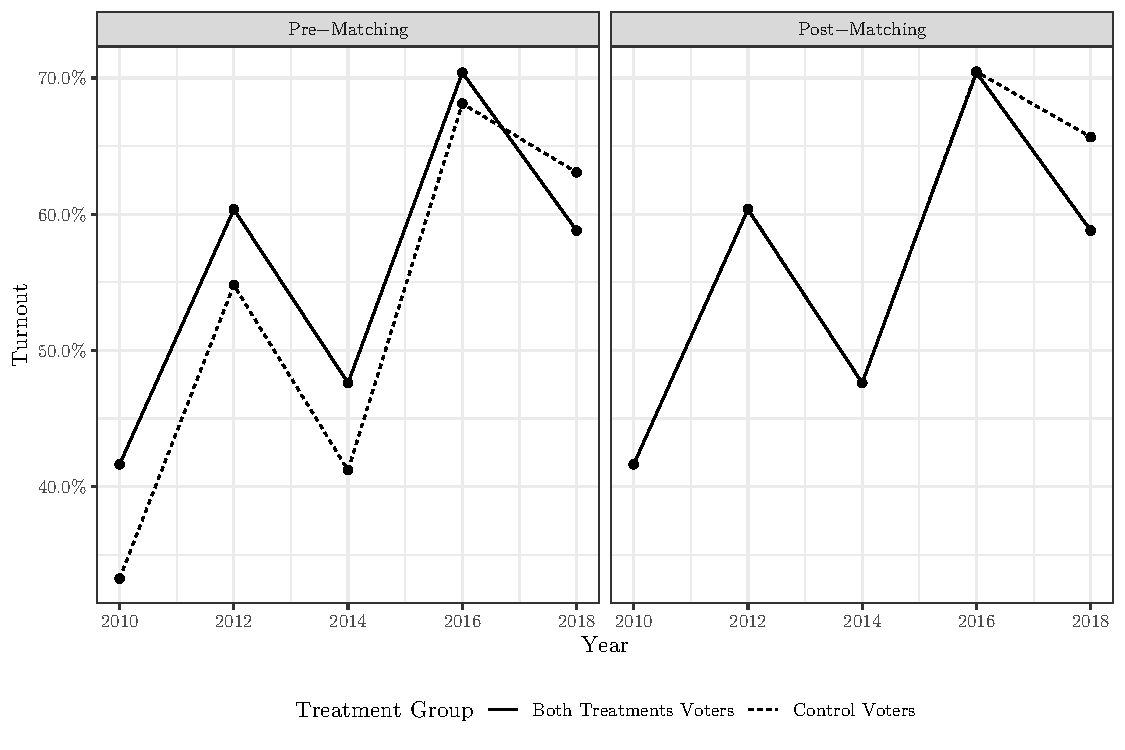
\includegraphics{hurricane_michael_files/figure-latex/full-to-chunk-1} 

}

\caption{\label{fig:full-to}General Election Turnout for Treated and Control Voters, 2010 -- 2018}\label{fig:full-to-chunk}
\end{figure}

Table \ref{tab:full-dind} formalizes Figure \ref{fig:full-to} into a differences-in-differences regression specification. We employ an ordinary least squares specification.\footnote{Although the dependent variable here is binary --- it takes the value 0 if a voter does not participate, and 1 if she does --- the coefficients produced by logistic regressions in the difference-in-differences context are largely uninterpretable. We thus use a linear specification here. When the models are estimated using a logistic specification, the treatment effect is consistent.} The dependent variable takes the value 1 if a voter cast a ballot in a given year, and 0 if she did not. Model 1 includes only three variables in addition to the constant. \emph{Treated} measures the gap between treated and control voters in the 2010 -- 2016 period. \emph{2018} measures the increase in turnout observed among control voters in 2018, while \emph{Treated × 2018} measures whether turnout in 2018 departed further or less from the baseline for the treated voters than the control voters. Model 2 includes the same variables, but also includes the characteristics on which the voters were matched. Model 3, finally, also includes measures for congressional district competitiveness. Because this variable is ``downstream'' of treatment --- that is to say, the effect of the hurricane could have impacted the competitiveness of certain races --- it is not included in the first two models. It should be noted that each of the treated voters lived in uncontested congressional districts. Robust standard errors are clustered at the level of the match (Abadie and Spiess \protect\hyperlink{ref-Abadie2019}{2019}).

\begin{singlespace}
\input{"../temp/dind_full.tex"}
\end{singlespace}

The coefficient on \emph{Treated × 2018} in Table \ref{tab:full-dind} indicates that Hurricane Michael had a substantial depressive effect in 2018 among the treated voters. Each model estimates that the overall effect --- including individual and administrative effects --- was -8.4 percentage points. Multiplied across the nearly 200 thousand registered voters in the treated counties indicates that some 16 thousand ballots went uncast due to the hurricane --- a major effect in a year when a statewide senate race was decided by 10,033 votes.

\hypertarget{identifying-adminstrative-effects}{%
\subsection*{Identifying Adminstrative Effects}\label{identifying-adminstrative-effects}}
\addcontentsline{toc}{subsection}{Identifying Adminstrative Effects}

As discussed above, our primary strategy for isolating the administrative effects of the hurricane on turnout involves leveraging random assignment around county borders in the Florida panhandle in a double-matched triple-differences specification. This specification involves matching voters in treated counties to voters in neighboring, untreated counties. This allows us to control for weather effects, while letting the administrative context vary. Treated and these matched, ``primary control voters'' are then matched to voters elsewhere in the state, allowing us to test the overall effect of the storm on turnout. By comparing the treatment effect for the primary control voters to the treatment voters in a triple-differences framework, we can decompose the individual-level effects from the administrative effects of Hurricane Michael.

We begin by identifying all voters who lived within two miles of a county with a different treatment status. Figure \ref{fig:map} shows the map of counties in the region. The eight treated counties are drawn in a medium gray, and the untreated border counties are drawn in dark gray. All treated and control voters come from the light gray buffer, which extends for two miles on either side of the border between a treated and untreated county. There are not voters in Gulf, Calhoun, or Franklin Counties who live within two miles of an untreated county.

\begin{figure}[H]

{\centering 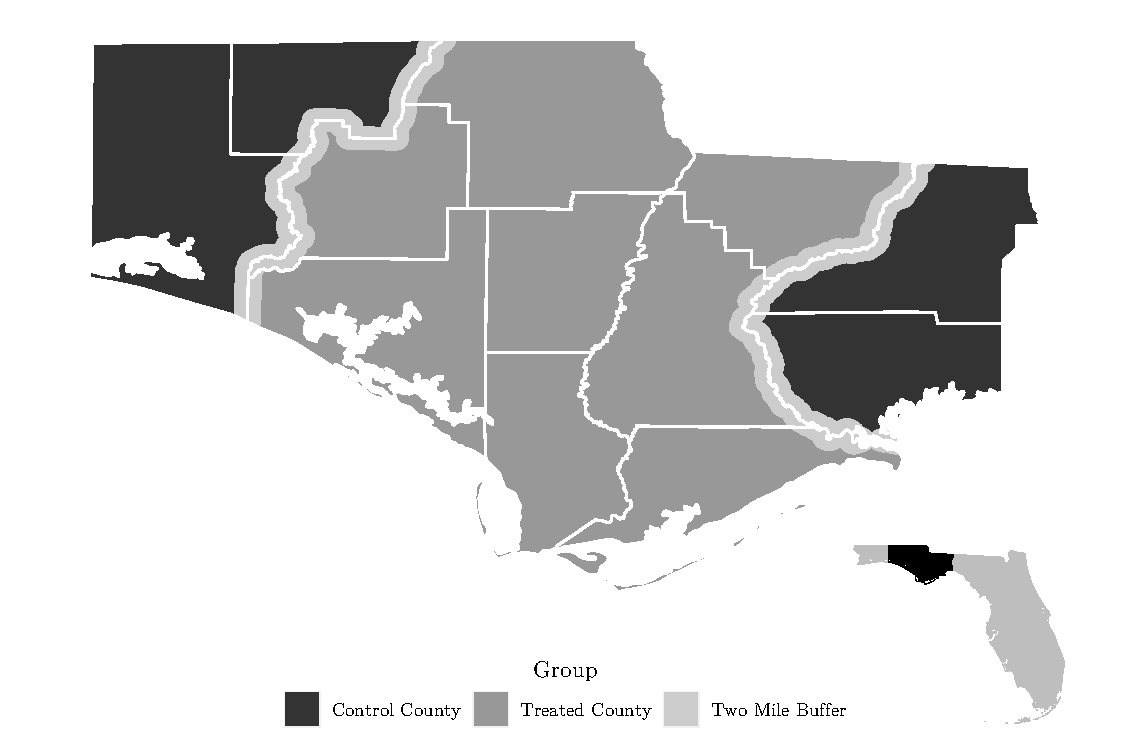
\includegraphics{hurricane_michael_files/figure-latex/map-chunk-1} 

}

\caption{\label{fig:map}Treated and Control Counties with Two Mile Buffer}\label{fig:map-chunk}
\end{figure}

Each voter inside the buffer in a treated county is matched with one voter in the buffer in an untreated county, once again using the genetic matching algorithm developed by Sekhon (\protect\hyperlink{ref-Sekhon2011}{2011}). These matches serve as our primary control voters. Ties are not broken, which means that some treated voters are assigned multiple primary control voters; the weights used in the regressions below are adjusted accordingly.

In some cases, voters on either side of the border are in different congressional districts. This would pose a problem if these races were contested thanks to the potentially mobilizing effects of house races, but the entire buffer falls in uncontested congressional districts. This means that treated and untreated voters are not facing differential mobilization from congressional races. As before, we match on individual- and neighborhood-level characteristics. Importantly, we match treated and untreated voters using their latitude and longitude to ensure that matches live in close proximity to one another. Table \ref{tab:balance-ll} presents the results of this matching exercise.

\begin{singlespace}
\begin{table}[H]

\caption{\label{tab:balance-tab-ll}\label{tab:balance-ll} Balance Table for Border Buffer Matching}
\centering
\resizebox{\linewidth}{!}{
\begin{tabular}[t]{lllllrrrr}
\toprule
\multicolumn{1}{c}{ } & \multicolumn{2}{c}{Means: Unmatched Data} & \multicolumn{2}{c}{Means: Matched Data} & \multicolumn{4}{c}{Percent Improvement} \\
\cmidrule(l{3pt}r{3pt}){2-3} \cmidrule(l{3pt}r{3pt}){4-5} \cmidrule(l{3pt}r{3pt}){6-9}
 & Treated & Control & Treated & Control & Mean Diff & eQQ Med & eQQ Mean & eQQ Max\\
\midrule
\%White & 74.9\% & 82.7\% & 74.9\% & 74.9\% & 100.00 & 100.00 & 100.00 & 100.00\\
\% Black & 20.7\% & 12.1\% & 20.7\% & 20.4\% & 96.51 & 96.63 & 96.63 & 96.63\\
\% Latino & 1.5\% & 1.6\% & 1.5\% & 1.3\% & -153.02 & -144.51 & -144.51 & -144.51\\
\% Asian & 0.4\% & 0.5\% & 0.4\% & 0.4\% & 100.00 & 100.00 & 100.00 & 100.00\\
\% Female & 53.4\% & 52.8\% & 53.4\% & 53.4\% & 98.07 & 98.13 & 98.13 & 98.13\\
\% Male & 45.4\% & 45.7\% & 45.4\% & 45.5\% & 76.18 & 76.98 & 76.98 & 76.98\\
Age & 52.536 & 51.612 & 52.536 & 52.446 & 90.26 & 72.06 & 70.58 & 60.06\\
\% Democrat & 44.2\% & 38.8\% & 44.2\% & 44.2\% & 100.00 & 100.00 & 100.00 & 100.00\\
\% Republican & 41.9\% & 45.0\% & 41.9\% & 41.9\% & 99.47 & 99.48 & 99.48 & 99.48\\
\% with Some College & 63.8\% & 66.7\% & 63.8\% & 65.0\% & 58.28 & 43.39 & 26.07 & -17.56\\
Median Income & \$47,598 & \$49,407 & \$47,598 & \$47,242 & 80.30 & -26.88 & -17.50 & 11.06\\
\bottomrule
\end{tabular}}
\end{table}
\end{singlespace}

The match procedure improves the balance between treated and primary control voters substantially for 10 of the 11 characteristics listed in Table \ref{tab:balance-ll}. The share Latino --- the only characteristic to go unimproved --- is below 2 percent for both groups and the difference is unlikely to cause any problems. Although latitudes and longitudes are not displayed in the table, the average treated voter lives just 8.5 miles from her primary control voter. This distance satisfies our assumption that treated and primary control voters faced the same weather effects from the hurricane. Figure \ref{fig:ll-to} makes clear that the parallel trends assumption is satisfied for post-matching treated and primary control voters. Turnout patterns in the two groups track very closely. In the pre-treatment period, treated voters turned out at slightly higher rates than their primary controls in midterm years. To the extent this impacts our analysis, it will make any estimated negative treatment effect in 2018 conservative.

\begin{figure}[H]

{\centering 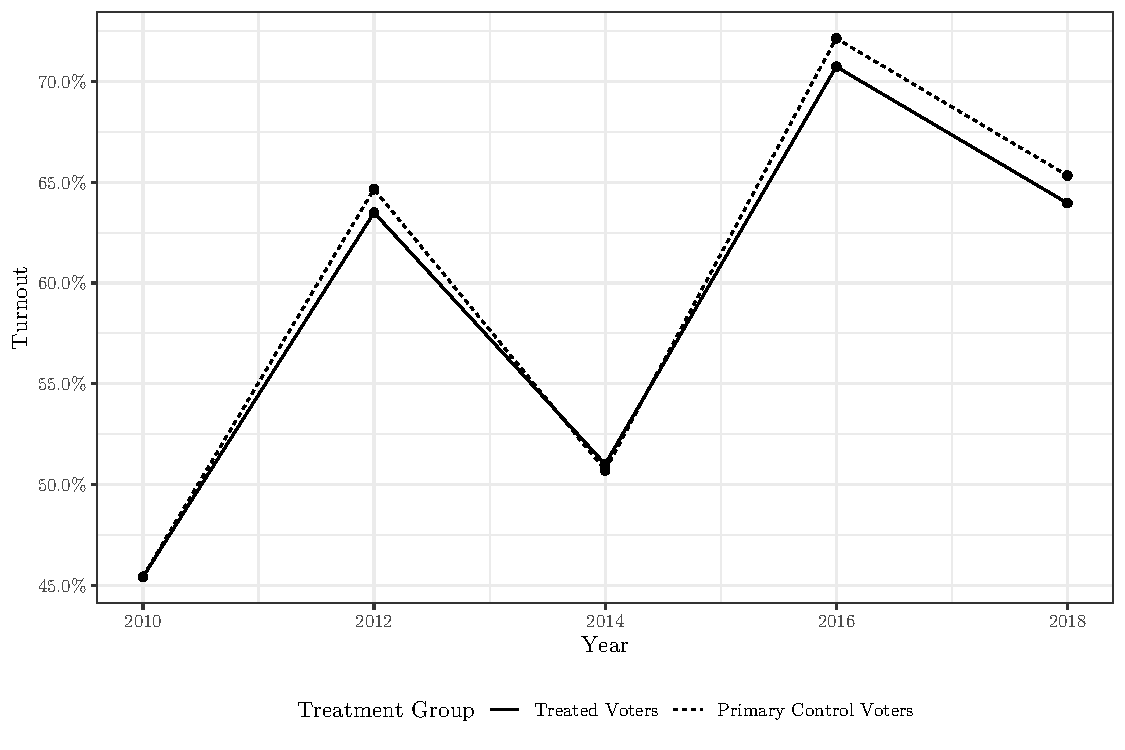
\includegraphics{hurricane_michael_files/figure-latex/ll-to-chunk-1} 

}

\caption{\label{fig:ll-to}General Election Turnout for Treated and Primary Control Voters, 2010 -- 2018}\label{fig:ll-to-chunk}
\end{figure}

Once our set of treated and primary control voters has been identified, each of these voters is matched with five other voters that lived in neither the treated nor the immediately surrounding counties. For ease of notation, the combined set of treated and primary control voters will henceforth be refered to as ``Panhandle voters,'' while ``treated'' voters will distinguish Panhandle voters in treated counties from Panhandle voters in other counties. The use of ``Panhandle'' is a slight misnomer: it excludes Escambia, Santa Rosa, and Okaloosa Counties which are certainly part of the Florida Panhandle, as well as Jefferson County and others to its east which are sometimes considered part of the panhandle. Nevertheless, we adopt this shorthand for referring to the treated counties and their neighbors.

This matching procedure follows the same steps detailed in the Overall Turnout Effects section of this paper. Table \ref{tab:balance-secondary} presents the results of the secondary match. We improve along all characteristics.

\begin{singlespace}
\begin{table}[H]

\caption{\label{tab:balance-tab-ll2}\label{tab:balance-secondary} Balance Table for Secondary Match}
\centering
\resizebox{\linewidth}{!}{
\begin{tabular}[t]{lllllrrrr}
\toprule
\multicolumn{1}{c}{ } & \multicolumn{2}{c}{Means: Unmatched Data} & \multicolumn{2}{c}{Means: Matched Data} & \multicolumn{4}{c}{Percent Improvement} \\
\cmidrule(l{3pt}r{3pt}){2-3} \cmidrule(l{3pt}r{3pt}){4-5} \cmidrule(l{3pt}r{3pt}){6-9}
 & Treated & Control & Treated & Control & Mean Diff & eQQ Med & eQQ Mean & eQQ Max\\
\midrule
\%White & 74.9\% & 62.3\% & 74.9\% & 74.9\% & 100.00 & 100.00 & 100.00 & 100.00\\
\% Black & 19.7\% & 13.1\% & 19.7\% & 19.7\% & 100.00 & 100.00 & 100.00 & 100.00\\
\% Latino & 1.8\% & 17.4\% & 1.8\% & 1.8\% & 100.00 & 100.00 & 100.00 & 100.00\\
\% Asian & 0.5\% & 2.0\% & 0.5\% & 0.5\% & 100.00 & 100.00 & 100.00 & 100.00\\
\% Female & 53.0\% & 52.4\% & 53.0\% & 53.0\% & 100.00 & 100.00 & 100.00 & 100.00\\
\% Male & 45.6\% & 44.9\% & 45.6\% & 45.6\% & 100.00 & 100.00 & 100.00 & 100.00\\
Age & 52.403 & 52.489 & 52.403 & 52.398 & 93.30 & 90.74 & 88.85 & 80.02\\
\% Democrat & 43.6\% & 37.1\% & 43.6\% & 43.6\% & 100.00 & 100.00 & 100.00 & 100.00\\
\% Republican & 41.3\% & 35.0\% & 41.3\% & 41.3\% & 100.00 & 100.00 & 100.00 & 100.00\\
\% with Some College & 63.8\% & 75.1\% & 63.8\% & 63.8\% & 99.94 & 99.79 & 98.00 & 74.54\\
Median Income & \$47,154 & \$62,941 & \$47,154 & \$47,003 & 99.05 & 97.51 & 93.67 & 73.01\\
\bottomrule
\end{tabular}}
\end{table}
\end{singlespace}

Figure \ref{fig:second-parallel} demonstrates that the parallel trends assumption generally holds: turnout among the secondary controls tracks neatly with the turnout of the Panhandle voters prior to 2018. A visual inspection of Figure \ref{fig:second-parallel} surprisingly does not reveal any major change in turnout in 2018 for all Panhandle voters relative to their matches in the rest of the state.

\begin{figure}[H]

{\centering 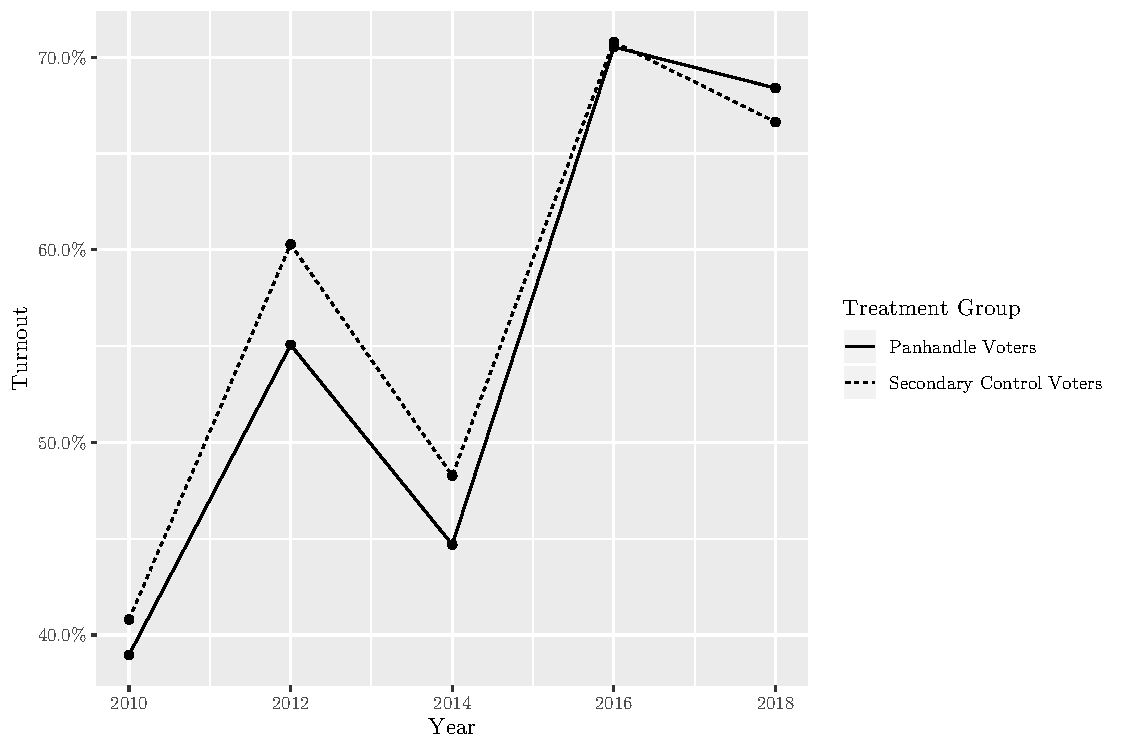
\includegraphics{hurricane_michael_files/figure-latex/second-parallel-chunk-1} 

}

\caption{\label{fig:second-parallel}General Election Turnout for Panhandle and Secondary Match Voters, 2010 -- 2018}\label{fig:second-parallel-chunk}
\end{figure}

Disentangling the administrative and individual effects of the storm requires the estimation of the triple-differences model. This model is estimated by Equation (1).

\begin{gather}
\label{eq:1}
v_{it}=\beta_0+\beta_1Panhandle_{i}+\beta_22018_{t}+\beta_3Panhandle_{i}\times 2018_{t} + \nonumber \\
\beta_4Treated_{i} + \beta_5Treated_{i}\times 2018_{t} + \beta_6Secondary Control Group 1_{i} + \\
\beta_7Midterm_{t} + \beta_8Panhandle_{i}\times Midterm_{t} + \beta_9Treated_{i}\times Midterm_{t} + \nonumber \\
\delta{Z}_{i} + \mathcal{E}_{it}. \nonumber
\end{gather}

Individual \emph{i}'s turnout (\emph{v}) in year \emph{t} is a function of the year and their location. In the equation, \emph{b\textsubscript{1}Pandhandle\textsubscript{i}} measures the historical difference between voters in the panhandle (both treated and matched, untreated individuals) and the rest of the state. \emph{b\textsubscript{2}2018\textsubscript{t}} measures the statewide change in turnout in 2018 from the baseline, while \emph{b\textsubscript{3}Panhandle\textsubscript{i} × 2018\textsubscript{t}} tests whether turnout changed differently in 2018 in the panhandle than it did elsewhere. \emph{b\textsubscript{3}Panhandle\textsubscript{i} × 2018\textsubscript{t}}, therefore, is our estimation of the individual-level, or weather related, effect of the hurricane. \emph{b\textsubscript{4}Treated\textsubscript{i}} measures the historical difference between treated and control observations in the buffer, and \emph{b\textsubscript{5}Treated\textsubscript{i} × 2018\textsubscript{t}} tests whether the change in turnout in 2018 was different for voters living in the treated counties than for their matched controls in the panhandle. We also test whether the secondary control voters for the treatment group had higher or lower turnout than the other set of secondary control voters using \emph{b\textsubscript{6}SecondaryControlGroup1\textsubscript{i}} term.

We also allow for the possibility that there are different gaps between groups of voters in midterm and presidential years. As Figure \ref{fig:ll-to} indicates, the primary control voters historically had higher levels of turnout than the treated voters in presidential years, but that gap disappears in midterm years. These potential differences are captured in the variables \emph{b\textsubscript{7}Midterm\textsubscript{t}}, \emph{b\textsubscript{8}Panhandle\textsubscript{i} × Midterm\textsubscript{t}}, and \emph{b\textsubscript{9}Treated\textsubscript{i} × Midterm\textsubscript{t}}. Finally, the matrix \emph{\(\delta\)Z\textsubscript{i}} contains the individual- and neighborhood-level characteristics on which the match was performed, included in some of the models.

Each treated voter and her subsequent matches are also weighted to account for the share of their county's population in the 2-mile buffer, as well as their county's total population. Bay County, for instance, accounts for 47 percent of the population of all 8 treated counties; treated Bay County voters and their matches, therefore, are weighted to account for 47 percent of the triple-difference panel.

Table \ref{tab:trip-diff} presents the results of this model, again fit using an ordinary least squares specification. Model 1 includes only the dummies discussed above, while Model 2 includes all the covariates on which the matching procedures were performed. Model 3 also includes estimates for congressional district competitiveness in 2018. Robust standard errors are clustered at the level of the original treated voter from which the primary and secondary controls arise.

\begin{singlespace}

\input{"../temp/triple_diff.tex"}
\end{singlespace}

The coefficients on \emph{Panhandle} in Table \ref{tab:trip-diff} demonstrate that prior to 2018, Panhandle voters generally saw turnout that was 4.7 percentage points above the turnout of the secondary controls; the nonsignificance of \emph{Treated} and (generally) \emph{Secondary Control Group 1} indicates that turnout between treated and primary control voters, and between the two groups of secondary controls, were not meaningfully different in the base periods. Coefficients for \emph{2018} indicate that turnout was higher in 2018 for the secondary control voters than in the base period; however, because we do not include explicit controls for midterm and presidential years, it is not directly interpretable.

Each model in Table \ref{tab:trip-diff} indicates that turnout in 2018 did not change differently for primary control voters than for secondary control voters; in each model, the coefficient on \emph{Panhandle × 2018} is small and nonsignificant. It seems that these voters lived far enough from the center of the hurricane's destruction to avoid having their turnout affected.

The coefficients on \emph{Treated × 2018}, however, indicate that turnout was depressed for treated voters who lived just inside counties covered by the executive order (after controlling for changed turnout among primary and secondary control voters). Because the treated and primary control voters faced the same weather --- and therefore individual effects --- of the storm, this loss in turnout can be attributed to the administrative problems faced by the treated voters. Each model estimates that this effect was -3.1 percentage points.

This estimated administrative effect can only be understood as the treatment effect on the treated; it does not necessarily reflect the administrative effect faced by \emph{all} voters in the treated counties. And, in fact, because there are no treated voters from Gulf, Calhoun, or Franklin Counties included in these models, it is likely not fully representative of the experience faced by all voters. Nevertheless, this 3.1 percentage point decrease in turnout from administrative effects is large relative to the overall depressive effect of Hurricane Michael estimated in Table \ref{tab:full-dind} (-8.4 percentage points). This indicates that the administrative effects likely played a substantial role in the overall depressed turnout in these counties.

\hypertarget{where-did-the-ballots-go}{%
\section*{Where Did the Ballots Go?}\label{where-did-the-ballots-go}}
\addcontentsline{toc}{section}{Where Did the Ballots Go?}

Having established that turnout was substantially depressed in the treated counties and that a non-trivial amount of the depression arose from administrative costs, we turn to a new question: where did these ballots go? We know that Executive Order 18-283 loosened restrictions on early and mail balloting; we therefore expect that, relative to the rest of the state, a higher share of ballots in the treated counties cast their ballots in one of these ways.

We return to the matches produced earlier in this paper, where \emph{every} voter in the treated counties was matched with five voters elsewhere in the state (but in neither treated nor neighboring counties). Figure \ref{fig:vote-mode} demonstrates the share of registered voters that cast a ballot either at the polling place, early in person, or absentee. In each case, the denominator is the number of registered voters in 2018.

\begin{figure}[H]

{\centering 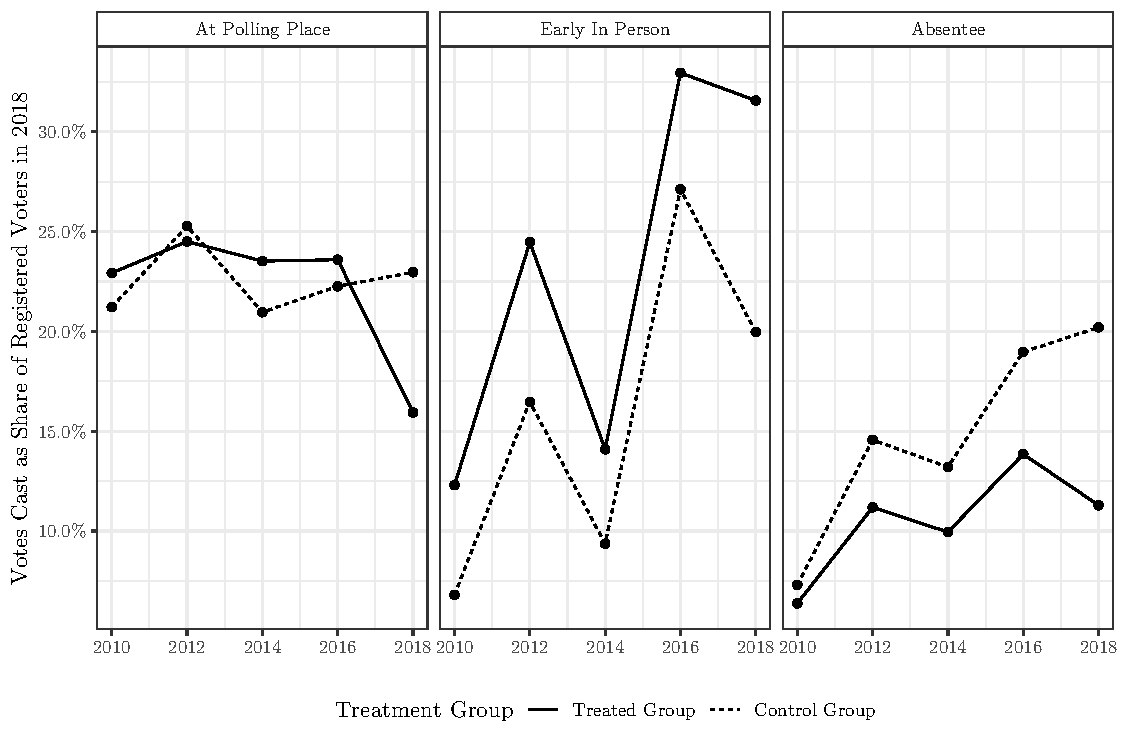
\includegraphics{hurricane_michael_files/figure-latex/vote-mode-chunk-1} 

}

\caption{\label{fig:vote-mode}Share of Voters Participating by Vote Method, 2010 -- 2018}\label{fig:vote-mode-chunk}
\end{figure}

Figure \ref{fig:vote-mode} makes clear that the decline in turnout was a product of lower turnout on election day, and via absentee voting. In fact, turnout among early voters appears to have been \emph{higher} in 2018 than would have been expected based on past behavior and the control voters' participation method in 2018.

The decrease in participation via absentee ballots prompts a follow-up question: the executive order should have made it far easier to vote absentee. Why, then, did a much lower share of voters vote using this method?

To understand why this is the case, we turn to data from the Election Assistance Commission's Election Administration and Voting Survey (EAVS). The EAVS asks election administrators a host of questions after each federal election --- including, importantly, the number of absentee ballots requested. We specifically use EAVS from 2016 and 2018 to understand the changes in the number of absentee ballots requested. In Figure \ref{fig:eavs} we plot the change in the percentage of registered voters who requested an absentee ballot in the two years for each county in Florida. In Palm Beach County, for instance, 19.6 percent of registered voters requested an absentee ballot in 2016, while 23.0 percent did so in 2018. The difference for Palm Beach County in Figure \ref{fig:eavs} is therefore 3.5 percentage points.\footnote{This is not 3.4 percentage points due to rounding.}

\begin{figure}[H]

{\centering 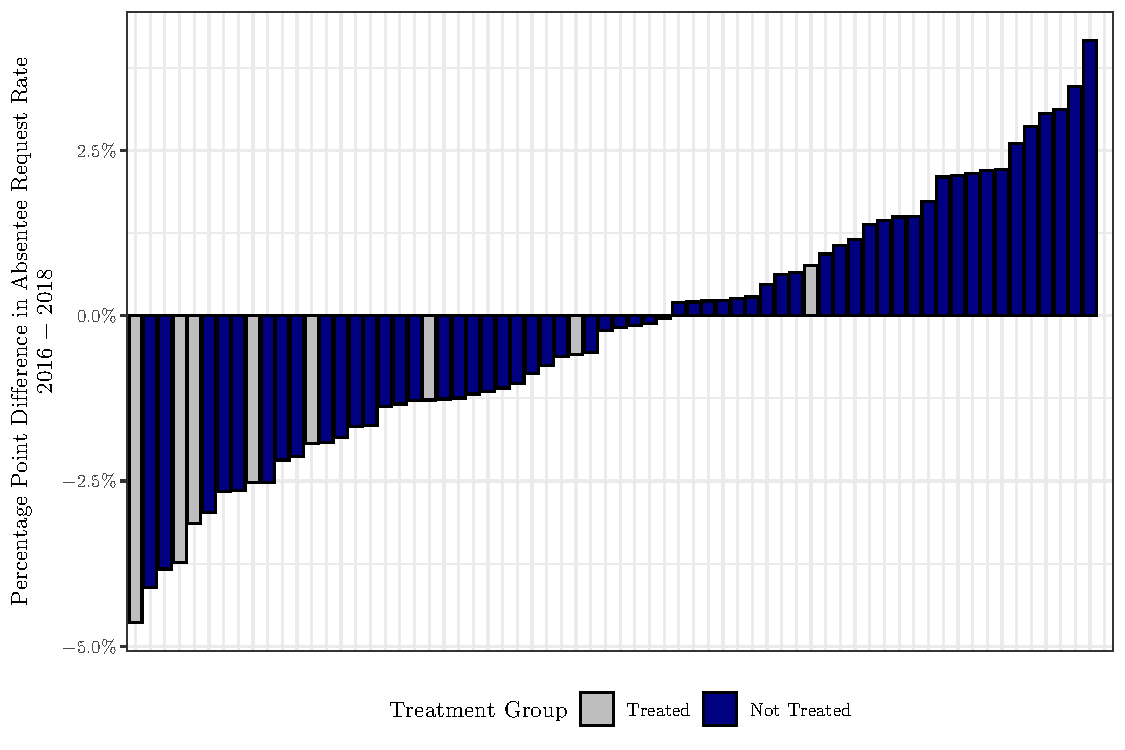
\includegraphics{hurricane_michael_files/figure-latex/eavs-chunk-1} 

}

\caption{\label{fig:eavs}Change in Absentee Ballot Request Rate, 2016 -- 2018}\label{fig:eavs-chunk}
\end{figure}

Sixty-six counties in Florida reported their absentee request rate in both 2016 and 2018. Of the ten counties where the request rate declined by the most, four were treated by the executive order. There were 29 counties where the share of registered voters who requested an absentee ballot increased between 2016 and 2018; just one of the treated counties, however, saw an increase. It appears that Hurricane Michael led to a substantial decrease in the request of absentee ballots. This is despite the fact that Executive Order 18-283 reduced the administrative hurdles to sending ballots to addresses other than the one listed on the voter rolls. It appears that the loosened restrictions were not well communicated to voters throughout the treated counties.

\begin{singlespace}
\input{"../temp/multinom.tex"}
\end{singlespace}

\hypertarget{discussion-and-conclusion}{%
\section*{Discussion and Conclusion}\label{discussion-and-conclusion}}
\addcontentsline{toc}{section}{Discussion and Conclusion}

Election Day in the United States consistently falls near the end of hurricane season. Hurricane Michael made landfall on October 10, 2018, less than a month before the highest-turnout midterm election in a century. Superstorm Sandy struck New York and New Jersey just days before the midterm elections in 2012, wreaking immense havoc. Hurricane Matthew struck the Southeastern United States weeks before the 2016 presidential election, killing dozens and causing more than \$2.5 billion in damages. Mann and Emanuel (\protect\hyperlink{ref-Mann2006}{2006}) and others have linked Atlantic hurricanes to climate change, indicating that these disruptions to election day activity are likely to increase in coming years. Understanding how storms of these nature impact turnout --- and whether state response is sufficient to recoup turnout --- is therefore vitally important, particularly in swing states such as Florida and North Carolina.

The 2020 election will face a different sort of disruption: as the novel coronavirus upends voting across the country, it is becoming clear that many voters will avoid physical polling places, opting instead to vote by mail or to simply abstain. In response to the threat posed by COVID-19 to voting, some states such as New York (Vielkind \protect\hyperlink{ref-Vielkind2020}{n.d.}) have moved to loosen restrictions on mail balloting in their primaries --- just as Florida did in the parts of the state hardest-hit by Hurricane Michael before the 2018 general election. Although COVID-19 looks much different than a hurricane, its effects on election administration promise to share many similarities. We need to look no further than Milwaukee, Wisconsin's primary election experience to see the similarities. Although Milwaukee generally has 180 in-person voting sites, these sites were consolidated to just 5 (Herndon \protect\hyperlink{ref-Herndon2020}{2020}). Whether polling places are shuttered due to structural damage or a public health crisis, their closures impose costs on voters.

As this paper demonstrates, the Florida's response to Hurricane Michael was not particularly effective: although Governor Scott increased access to mail voting in eight counties, mail balloting use in these areas actually \emph{dropped} relative to the rest of the state. Of course, mail balloting might have dropped by even more in the absense of the Executive Order; we cannot estimate the counterfactual. Nevertheless, Figures \ref{fig:vote-mode} and \ref{fig:eavs} indicate that the executive order probably did not shift voters to use the loosened mail voting option. Moreover, our double-matched triple-differences model indicates that the hurricane's administrative effect on turnout, net of the executive order, was -3.1 percentage points.

This is disheartening. Not only did the executive order fail to combat the negative individual-level effects of the hurricane on turnout; it did not even come close to mitigating the administrative effects. Clearly, loosening restrictions on where mail ballots could be sent and how they could be returned was not enough. Although the administrative effect on turnout would likely have been larger in the absence of the executive order, the net administrative effects were nonetheless substantial.

The data at hand cannot explain why the executive order was ineffective at neutralizing the administrative effects of the hurricane. The timing of the executive order, however, might shed some light. Although the hurricane made landfall on October 10, the executive order was not signed until more than a week later, on October 18 --- fewer than three weeks before the November 6 general election. This left little time for an effective public education campaign, perhaps limiting the number of voters who learned and took advantage of the changed rules. We found very few news articles detailing the changes and making the information easily available to voters (but see \emph{WJHG - Panama City} \protect\hyperlink{ref-WJHG2018}{2018}; Vasquez \protect\hyperlink{ref-Vasquez2018}{2018}; McDonald \protect\hyperlink{ref-McDonald2018}{2018}; Fineout \protect\hyperlink{ref-Fineout2018}{2018}), and what information did get published often listed only relocated polling places with no information about loosened mail voting restrictions (see, for instance, \emph{Gadsden Times} \protect\hyperlink{ref-gadsdentimes2018}{2018}). It is possible, of course, that local televised news communicated the changes to viewers; however, based on our search of published information, that information would have been difficult to find for voters who missed the televised news. We found no evidence that the Florida Times-Union (the largest paper in Northern Florida) or the Tampa Bay Times (the largest paper in the state) published any articles detailing the changes brought about by the executive order.

If election administrators do not look to past crises to understand how voters will respond, the administrative effects of the novel coronavirus on general election turnout this fall might be large. Future research will no doubt leverage pre-existing administrative regimes to understand the sorts of voting environments least susceptible to disruption from the coronovirus --- but such research will necessarily be backward looking. The experience of Hurricane Michael, on the other hand, gives us important insight about how an emergency that closes polling places will structure turnout. Executive Order 18-283 makes clear that simply loosening mail voting restrictions will not result in a wholesale adoption of vote-by-mail.

The novel coronavirus will perhaps lower turnout even if election administrators respond perfectly. Voting might be low on a list of priorities for individuals who are caring for ailing loved ones, grieving, or dealing with economic crises. Nevertheless, COVID-19 will also pose administrative hurdles to voting: consolidated or relocated polling places, reliance on a vote-by-mail system unfamiliar to many voters, or longer wait times as the number of voters allowed into a polling place at once might all reduce turnout. As administrators consider easing vote-by-mail restrictions, they must look to the case of Florida in 2018. More must be done than simply change the rules; otherwise, the administrative effects of COVID-19 will magnify the individual effects of this public health crisis on voter turnout.

\newpage

\hypertarget{references}{%
\section*{References}\label{references}}
\addcontentsline{toc}{section}{References}

\hypertarget{refs}{}
\begin{cslreferences}
\leavevmode\hypertarget{ref-Abadie2019}{}%
Abadie, Alberto, and Jann Spiess. 2019. ``Robust Post-Matching Inference.'' \emph{Working Paper.}

\leavevmode\hypertarget{ref-Fineout2018}{}%
Fineout, Gary. 2018. ``Florida to Bend Voting Rules in Counties Hit by Hurricane.'' \emph{Northwest Florida Daily News}, October 18, 2018. \url{https://www.nwfdailynews.com/news/20181018/florida-to-bend-voting-rules-in-counties-hit-by-hurricane}.

\leavevmode\hypertarget{ref-gadsdentimes2018}{}%
\emph{Gadsden Times}. 2018. ``Changes in Polling Places at Three Locations,'' October 30, 2018. \url{https://www.gadsdentimes.com/news/20181030/changes-in-polling-places-at-three-locations}.

\leavevmode\hypertarget{ref-Herndon2020}{}%
Herndon, Astead W. 2020. ``They Turned Out to Vote in Wisconsin During a Health Crisis. Here's Why.'' \emph{The New York Times: U.S.}, April 7, 2020. \url{https://www.nytimes.com/2020/04/07/us/politics/wisconsin-democratic-voters.html}.

\leavevmode\hypertarget{ref-Mann2006}{}%
Mann, Michael E., and Kerry A. Emanuel. 2006. ``Atlantic Hurricane Trends Linked to Climate Change.'' \emph{Eos, Transactions American Geophysical Union} 87 (24): 233--41. \url{https://doi.org/10.1029/2006EO240001}.

\leavevmode\hypertarget{ref-McDonald2018}{}%
McDonald, Zack. 2018. ``Bay Voters Getting 5 'Mega Voting' Sites.'' \emph{Panama City News Herald}, October 23, 2018. \url{https://www.newsherald.com/news/20181023/bay-voters-getting-5-mega-voting-sites}.

\leavevmode\hypertarget{ref-Parks2018}{}%
Parks, Miles. 2018. ``After Hurricane Michael, Voting 'Is the Last Thing on Their Minds'.'' \emph{NPR.org}, October 25, 2018. \url{https://www.npr.org/2018/10/25/659819848/after-hurricane-michael-voting-is-the-last-thing-on-their-minds}.

\leavevmode\hypertarget{ref-Sekhon2011}{}%
Sekhon, Jasjeet S. 2011. ``Multivariate and Propensity Score Matching Software with Automated Balance Optimization: The Matching Package for R.'' \emph{Journal of Statistical Software} 42 (1): 1--52. \url{https://doi.org/10.18637/jss.v042.i07}.

\leavevmode\hypertarget{ref-Vasquez2018}{}%
Vasquez, Savannah. 2018. ``HURRICANE MICHAEL: How to Vote in Gulf County.'' \emph{The Star}, October 18, 2018. \url{https://www.starfl.com/news/20181018/hurricane-michael-how-to-vote-in-gulf-county}.

\leavevmode\hypertarget{ref-Vielkind2020}{}%
Vielkind, Jimmy. n.d. ``New Yorkers Can Vote by Absentee Ballot Because of Coronavirus.'' \emph{Wall Street Journal: US}. Accessed April 20, 2020. \url{https://www.wsj.com/articles/new-yorkers-can-vote-by-absentee-ballot-because-of-coronavirus-11586385420}.

\leavevmode\hypertarget{ref-WJHG2018}{}%
\emph{WJHG - Panama City}. 2018. ``Bay County Hurricane Michael Recovery Information,'' October 31, 2018. \url{https://www.wjhg.com/content/news/Bay-County--498037961.html}.
\end{cslreferences}

\end{document}
